\subsection{Typical \IOT Scenarios}
\label{sec:Motivation-Scenarios}

Figure \ref{fig:scenario} describes a typical instalment at Alice's smart home, the fictional character we use in our case study. Alice asked her technician to deploy simple devices: light sensors and bulbs to lighten the rooms; motion and door detectors to detect human activity; an alarm that produces a sound in case of emergency; and a toggle button installed in the balcony for security purposes. 

%In order to illustrate our proposal, we will use a hypothetical \IOT configuration depicted in Figure~\ref{fig:scenario} where Alice's apartment is represented with a set of sensors and actuators.
\begin{figure}%
	\centering  
	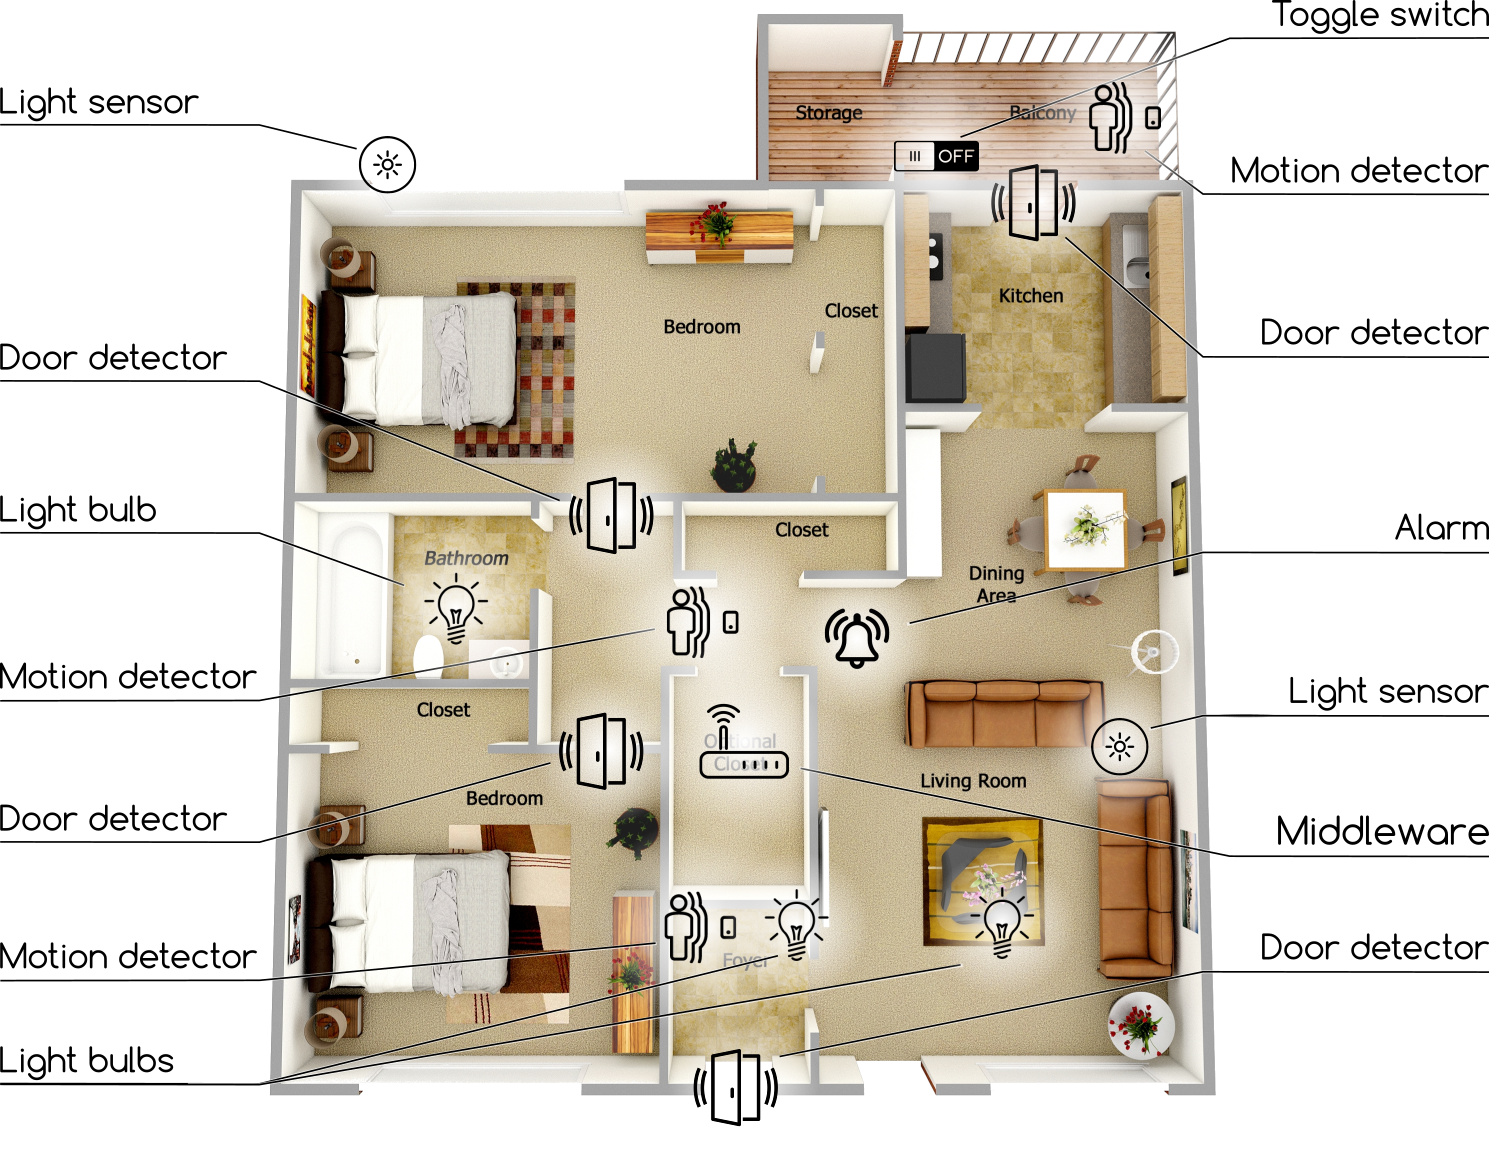
\includegraphics[width=.9\linewidth]{scenario.png}%
	\caption{Hypothetical Alice's \textit{smart-home} configuration of \IOT devices}%
	\label{fig:scenario}%
\end{figure}

Alice is interested in simple scenarios for her comfort and her little boy's security: she wants the entrance lights to automatically switch on to welcome her when she arrives home; 
%she likes her apartment to stay reasonably warm along the year; 
and since her boy often plays in the balcony, or sometimes wakes up at night and walks through the apartment, she needs to ensure he does not fall or injure himself.
Those scenarios seem already possible with the equipment she currently has: we will show how to implement them through a rule-based specification in Section \ref{sec:IoTDSL-BusinessRules}.

%This typical smart home configuration consists of light sensors and bulbs to handle the light in the apartment, motion and door detectors to verify the presence of persons, an alarm in case of emergency and a toggle switch on the balcony. Even if the amount of types of devices is rather limited, we can already highlight a set of features absolutely needed to describe the devices, network configuration and specify its dynamic aspects.

